\subsection{Advection--diffusion equations}
\label{sec: advection_diffusion}
In this section, we want to extend our stability analysis to the one-dimensional advection-diffusion equation
\begin{equation}\label{eq: A-D_equation}
u_t(x,t) + au_x(x,t) = du_{xx}(x,t), \quad a\ge0, \ d \ge 0,
\end{equation}
where $a$ is the coefficient of the advection term and $d$ the coefficient of the diffusion term. 
\subsubsection{FD discretization}
\label{sec: spatial_discretization}
By using the method of lines approach, we want to apply spatial discretizations to the spatial derivative operators, namely $\partial_x$ and $\partial_{xx}$, which represent respectively the advection and diffusion process. \\
With the common usage of a uniformed grid $\Omega_h=\left\{x_i \ : \ x_i = x_0 + ih, \ i \in \{0,\hdots , m\}\right\}$, the difference quotient just requires the values $x \in \Omega_h$. With given boundary values $u(x_0), \ u(x_m)$, this results in a linear system of equations, which can be embedded in a differential equation. 

\textbf{The advection term}
\vspace{2mm}
\\
In this section, we want to introduce the considered finite difference schemes for the discretization of the advection term in the advection-diffusion equation, i.e. the first spatial derivative $\partial_xu(x)$. One method of choice could consist of the already seen backward finite difference, because we assume $a\ge0$ in \eqref{eq: A-D_equation} and later discussed stability conditions require an upwind scheme in this direction. However, we have decided to abandon pure backward differences (i.e. $w_j(t)=\sum\limits_{k\le 0} c_kw_{j+k}$) due to other stability issues that arose in the process. In exchange, we want to introduce the more arbitrary discretizations as in \cite{Iserles1982} to provide better stability, as we will observe in later analysis.
\begin{definition}\mbox{}\\
	On a given spatial discretization $\Omega_h=\{x_0,\hdots, x_m\}$, we discretize the function $u(x)$ by $\{u(x_0), u(x_1), \hdots, u(x_m)\}\mapsto\{w_0, w_1, \hdots, w_m\}$ and introduce the arbitrary $[r,s]$- discretization to approximate $\partial_xu$ at $x_j$ by
	\begin{equation}\label{eq: r-s_scheme}
	\partial^{[r,s]}_h(u(x_j)) = \frac{1}{h} \sum\limits_{k=-r}^s \alpha_k w_{j+k}.
	\end{equation}
	We choose $r,\ s$ such, that $\alpha_{j-r}, \alpha_{j+s} \neq 0$ and call the set $\{x_{j-r}, \hdots, x_{j+s}\}$ the stencil of the discretization around $x_j$.
\end{definition}
It turns out, that the maximum order we can achieve with an $[r,s]$- discretization is $q=r+s$ and further, that this discretization is unique. It is also proven in \cite{Iserles1982} that these so-called $\textit{optimal-order}$ schemes of order $q$ are stable if and only if $s\le r \le s+2$ for $a>0$. We express these properties by the following theorems:
\begin{prop}\mbox{}\\
	For $r, \ s \ge0$, there exists an unique optimal-order scheme of order $q=r+s$. It is given by \eqref{eq: r-s_scheme} with the coefficients
	\begin{align*}
	\alpha_0&=\left\{ \begin{array}{cc}
	\sum\limits_{k=r+1}^s\frac{1}{k}, & s\ge r+1 \\
	0, & s=r \\
	\sum\limits_{k=s+1}^r\frac{1}{k}, & r\ge s+1 \\
	\end{array}
	\right. \\
	\alpha_k &= \frac{(-1)^{k+1}}{k}\cdot \frac{r!s!}{(r+k)!(s-k)!}, \quad -r\le k \le s, \ k\neq0.
	\end{align*}
\end{prop}

\begin{prop}\label{prop: optimal_order_stable}\mbox{}\\
	The only stable optimal-order schemes are $[r, r],\ [r, r+1]$ and $[r, r+2]$.
\end{prop}
The proofs of these statements can be found in \cite{Iserles1982}.\\
We also want to involve these schemes into our analysis. To rely further on upwind biased schemes, we will consider $[r, r +1]$ if we have talk about an odd optimal-order scheme and $[r, r+2]$ for an even scheme accordingly.
\\


\textbf{The diffusion term}
\vspace{2mm}
\\
In this section, we want to introduce the finite difference schemes for the diffusion term $\partial_{xx }u(x)$. For that matter, a suiting discretization is given by types of the central difference operator as previously seen. They can be constructed for arbitrary high (even) orders. The central finite difference schemes for the second spatial derivative which we will consider in this work are given in figure \ref{fig: CFD-schemes_first_deriv}.
\begin{figure}
	\centering
	\small
	\begin{tabular}[h]{|c|c|}
		\hline
		order & finite difference for $\partial_h^2(u(x_j))$\\
		\hline
		2 & $\frac{1}{h^2}\left(w_{j-1}-2w_j+w_{j+1}\right)$\\
		\hline
		4 & $\frac{1}{h^2}\left( -\frac{1}{12}w_{j-2} +\frac{4}{3}w_{j-1} -\frac{5}{2}w_j   +\frac{4}{3}w_{j+1}  -\frac{1}{12}w_{j+2}\right)$\\
		\hline
		6 & $\frac{1}{h^2}\left(\frac{1}{90}w_{j-3} - \frac{3}{20}w_{j-2} + \frac{3}{2}w_{j} - \frac{49}{18}w_{j} + \frac{3}{2}w_{j} - \frac{3}{20}w_{j+2} + \frac{1}{90}w_{j+3}\right)$\\
		\hline
		8 & $\frac{1}{h^2}\left(
		-\frac{1}{56}w_{j-4} + \frac{1}{420}w_{j-3} - \frac{1}{5}w_{j-2} + \frac{8}{5}w_{j-1} - \frac{205}{72}w_{j} + \frac{8}{5}w_{j+1} - \frac{1}{5}w_{j+2} + \frac{1}{420}w_{j+3} - \frac{1}{56}w_{j+4}
		\right)$\\
		\hline
	\end{tabular}
	\caption{Central finite difference discretizations $w_j$ approximating $u(x_j)$, \cite{fornberg_finite_difference}.}
	\label{fig: CFD-schemes_first_deriv}
\end{figure}
Analoge to the first derivative, the order of these schemes can be proven by taking the Taylor expansions of $u(x_j)$ and taking the difference with the respective spatial operator. 

\subsubsection{von Neumann Stabiity}
\label{sec: stability_theory_PDE}
To analyze the stability of the recent described methods, we take use of the von Neumann stability analysis for linear partial differential equations.\\

Briefly summarized, we take use of Fourier analysis to investigate the Fourier modes
\begin{equation*}\label{eq: fourier_modes}
w^n_j = v^ne^{ikx_j},
\end{equation*}
where $w^n_j$ is the discretization of $u(x_j, t_n)$ and $k$ the wavenumber and focus on the representation $v^n$. This works, because the $e^{(ikx)}$ are eigenfunctions of the differential operator $\partial_x$ and therefore for any linear differential operator. If we insert this in our discretized system, we reorder the terms to receive an equation of the form
\begin{equation}
\label{eq: ampfactor}
v^{n+1}=G(k, \Delta x, \Delta t, a, d)v^n.
\end{equation}
Thereby $G$ is called the amplification factor, which contains all information about the considered differential equation and the involved schemes. Because of our linear system, the here calculated amplification factor of the discretized scheme is the same as for the produced error of the method. This theory concludes in the following condition: 
\begin{prop}\textbf{Richtmyer condition}\\
	A finite difference scheme equipped with a time-stepping method is stable in the stability area $\Lambda$ if and only if there exists a constant $K$, such that
	\begin{equation*}
	\lvert G (k, \Delta x, \Delta t, a, d) \rvert \le 1+ K \Delta t
	\end{equation*}
	with $(k, \Delta x, \Delta t, a, d)\in \Lambda$. 
\end{prop}
Remark that for consistency, we included the parameters $a$ and $d$ into the dependency of $G$ to cover all advection-diffusion equations. When we evaluate the amplification factors numerically later on, we will probe the slightly more strict von Neumann condition $\lvert G (k, \Delta x, \Delta t, a, d) \rvert \le 1$ for stability. \\
This whole analysis gains its relevance based on the following statement.
\begin{theorem}\textbf{Lax-Richtmyer}\\
	A consistent finite difference scheme for a partial differental equation with a well-posed inital value problem is convergent if and only if its stable.
\end{theorem}
%%%%%%%%%%%%%%%%%
%Displaying Stability
%%%%%%%%%%%%%%%%%
To receive properties for the advection-diffusion equation, an analytical approach needs to solve a bunch of equations and is therefore not practical, especially if we take in consideration that we want to use the higher order ADER and DeC time marching methods and higher order spatial discretizations. \\
Hence, we will approach this numerically by evaluating the amplification factor, similar as we did with the stability functions in the ODE cases.
Before we can show and analyze these results, we have to discuss what is a good concept of displaying stability. This question arises out of the many existing variables. In contradiction to the ODE case, where the analysis is broken down to the Dahlquist test equation.
So recall, that the following analysis uses and is therefore restricted to the advection-diffusion equation
\begin{equation}
\partial_t y(x,t)+a\cdot \partial_x y(x,t)=d\cdot \partial_{xx }y(x,t), \quad a , \ d \ge 0.
\end{equation}
With given spatial discretizations $N(t,u)_i$ for the advection term and $L(t,u)_i$ for the diffusion term, we get a dependency on the mesh size $\Delta x=h$ and similar on the step size $\Delta t$ due to the time-marching method.
Combined with the advection coefficient $a$ and the diffusion coefficient $d$, we have four parameters, which variation should be taken in consideration while analyzing a specific method.\\
So for a given amplification factor $G$ dependent on $k, \Delta x, \Delta t, a, d$, where $k$ is again the wavenumber, we want to know when $\lvert G \rvert\le 1$ for all $k$. To achieve this numerically, it is sufficient to check this condition for a finite amount of wavenumbers
\begin{equation*}
k\in\{-n_0+1,n_0,\hdots,-1,0,1,\hdots,n_0,n_0+1\},
\end{equation*}
where $n_0$ is $"$large$"$.\\
\subsubsection{Displaying stability}
It is stated and numerically shown in \cite{TanChenShu_ImEx_Stability}, \cite{WangShuZhang_LDG1_2015},\cite{WangShuZhang_LDG_2016}, that several schemes as the local discontinuous Galerkin (LDG, see \cite{WangShuZhang_LDG1_2015},\cite{WangShuZhang_LDG_2016} for details) scheme and other finite difference schemes combined with an ImEx RK method are stable if the time step is upper bounded by some $\tau_0$. This $\tau_0$ is proportional to $\frac{d}{a^2}$, i.e. if $\Delta t\le\tau_0= c\cdot \frac{d}{a^2}$ for some $c>0$.
%%%%%%%%%%%%%%%%%
%C, D, E Approach
%%%%%%%%%%%%%%%%%
Considering the before mentioned parameters $\Delta x, \Delta t, a,d$, we introduce 2 new coefficients
\begin{equation}
C=\frac{a\Delta t}{\Delta x}, \quad D=\frac{d\Delta t}{{(\Delta x)}^2}.
\end{equation}
Therefore, for a given method solving the advection-diffusion equation, we receive  with \eqref{eq: ampfactor} the amplification factor
\begin{equation}
g=g(k,\Delta x, \Delta t, a,d)=g(k,C,D).
\end{equation}

Moreover using the coefficients $C$ and $D$, reveals an equivalent condition to \cite{TanChenShu_ImEx_Stability}, if we assume that the quotient
\begin{equation*}
E:=\frac{C^2}{D}= \frac{ \Delta t ^2 a^2 }{\Delta x^2} \frac{\Delta x^2}{d \Delta t} = \frac{a^2}{d}\Delta t
\end{equation*}
ist bounded by some constant $c$, because
\begin{equation*}
E= \frac{a^2}{d}\Delta t\le c \quad \Longleftrightarrow \quad \Delta t \le c \cdot \frac{d}{a^2}=\tau_0.
\end{equation*}
\LP{Introduce or change the notation for used methods?}
\begin{definition}\mbox{}\\
	To shorten up the notation, we denote the considered method for the advection-diffusion equation by
	\begin{equation*}
	[TMM,NODES,N, A_n,D_n],
	\end{equation*}
	where
	\begin{itemize}
		\item $TMM$ stands for the respective IMEX time-marching method, i.e. $DeC$, $ADER$, $sDeC$,
		\item $NODES$ stands for the used quadrature nodes for the TMM, i.e. $eq$ for equispaced or $GLB$ for Gauss-Lobatto,
		\item $N$ stands for the order of the considered time-marching method $TMM$,
		\item $A_n$ denotes order $n$ for the optimal-order stable stencils of proposition \ref{prop: optimal_order_stable} used for the advection part and
		\item $D_m$ denotes order $m$ for the central finite differences \ref{fig: CFD-schemes_first_deriv} used for the diffusion part.
	\end{itemize}
\end{definition}
\begin{example}\mbox{}\\
	To give an example of the behavior described just before, we will show in figure \ref{fig: exa_ImExDeC3_diff2_adv1} the stability areas for the $[DeC,eq,3, A_1,D_2]$ dependent on the coefficients $C/D$ on the left and $C/E$ on the right respectively. The black area is associated to the nonstable area, while the yellow displays the stable region.
	\begin{figure}[!h]
		\centering
		\begin{minipage}[t]{0.45\textwidth}
			\includegraphics[width=\textwidth]{plots/pde/exa_ImExDeC3_diff2_adv1CD.png}
			\centering
			Coefficients $C$ and $D$
		\end{minipage} 
		\begin{minipage}[t]{0.45\textwidth}
			\includegraphics[width=\textwidth]{plots/pde/exa_ImExDeC3_diff2_adv1CE.png}
			\centering
			Coefficients $C$ and $E$
		\end{minipage}
		\caption{Stability areas for the $[DeC,eq,3, A_1,D_2]$.}
		\label{fig: exa_ImExDeC3_diff2_adv1}
	\end{figure}
\end{example}

\begin{remark}\mbox{}\\
	With the previous derivations, we know of two conditions to obtain stability:
	\begin{itemize}
		\item The well known CFL-condition: If $C$ is lower than some constant $C_0$ dependent on the method, (e.g. $C<1=C_0$ for the explicit Euler as seen in example \ref{exa:VN_ImExEuler}) then the method is stable.
		\item The new numerically obtained condition, which we will denote by $E_0$-condition: If $E$ is lower than some constant $E_0$ dependent on the method, then the method is stable.
	\end{itemize}
	
	These two parameters $C$ and $E$ include all the remaining ones and show therefore a full picture.
\end{remark}

As we can see in figure \ref{fig: exa_ImExDeC3_diff2_adv1}, the nonstable area of this specific method seems to be bound to some axis-parallel lines $C=E_0$ and $E=C_0$. We will observe numerically, that these nonstable regions are indeed bound similary in most of our methods.\\
\begin{definition}\mbox{}\\
	Given the amplification factor $g(C,E)$ of a MOL to solve the AD-equation, we define the two stability parameters $C_0$ and $E_0$ by
	\begin{itemize}
		\item the maximum value $C_0$, so that $\lvert g(C_0,E)\rvert<1$ for every $E$ and
		\item the maximum value $E_0$, so that $\lvert g(C,E_0)\rvert<1$ for every $C$.
	\end{itemize}
\end{definition}
Therefore, the strategy we want to follow is to look at the areas of stability by evaluating the amplification factor $g(C,E)$ like in figure \ref{fig: exa_ImExDeC3_diff2_adv1} and, calculating the parameters $C_0$ and $E_0$ for our methods numerically if applicable.

Note, that the condition $E_0$ has the advantage to not depend on $\Delta x$ and makes it therefore possible to avoid the time step restriction of the CFL condition for methods which produce some $E_0$ remarkable larger than 0. \\
Further, it should be kept in mind that our numerical evaluations can just cover finite ranges. In our checks, we exceeded the here displayed limits for $E$ and $C$ to guarantee, that we do not receive instabilities in respect to the considered borders.
We also observed that all the considered results do not change if we set $n_0=10^3$. Due time-efficiency, we will use this value for every evaluation in the von Neumann stability analysis context for the rest of this work.
\subsubsection{Numerical analysis}
To distinguish the different orders this section, we apply different colors to the outer and inner bounds according to the legend figure \ref{fig: legend_a-d}. Remark that the colors are assigned to different types of orders, i.e. in one place to the order of the advection method, in the other place to the order of the time-marching and/or the diffusion method .
\begin{figure}[!h]
	\centering
	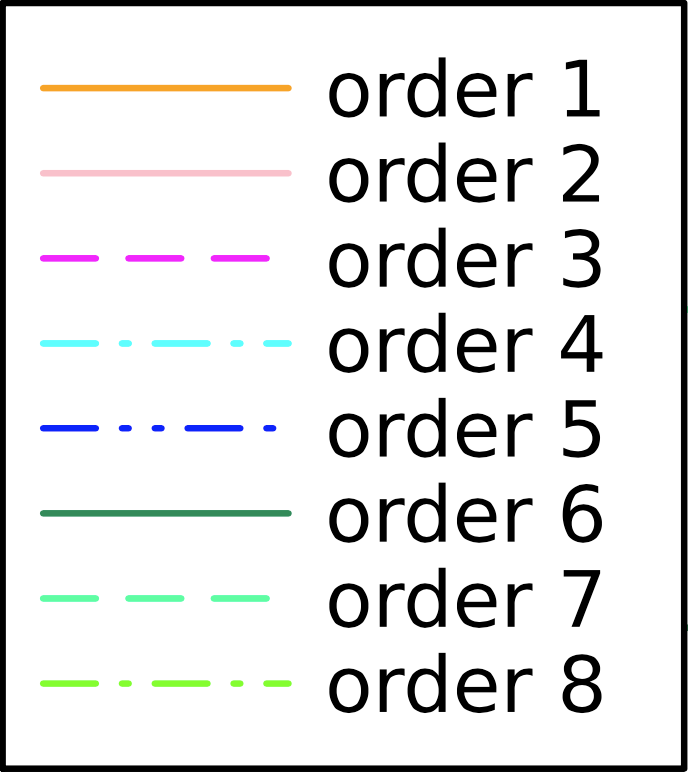
\includegraphics[width=0.18\textwidth]{pdepics/colors_a-d.png}
	\caption{Legend for the different orders.}
	\label{fig: legend_a-d}
\end{figure}\\
In figure \ref{fig: grp_adv1_diff2_GLB} are the contour lines of the stable and nonstable areas shown for the \\ $[DeC,GLB,k, A_1,D_2]$, $[sDeC,GLB,k, A_1,D_2]$, $[ADER,GLB,k, A_1,D_2]$, $k \in \{2,\hdots ,\}$. As in figure \ref{fig: exa_ImExDeC3_diff2_adv1}, the border separates between the stable region in the lower left and the unstable region in the upper right side of the respective image. We see for every method mostly a similar behavior. Increasing the order of the time marching method results in a higher region of stability and qualitative bigger values for $E_0$ and $C_0$ can be observed. 

\begin{figure}[!h]
	\centering
	\begin{minipage}[t]{0.32\textwidth}
		\includegraphics[width=\textwidth]{pdepics/IMEXDeC_GLB_diff2_adv1_C.png}
		\centering
		IMEX DeC
	\end{minipage} 
	\begin{minipage}[t]{0.32\textwidth}
		\includegraphics[width=\textwidth]{pdepics/IMEXsDeC_GLB_diff2_adv1_C.png}
		\centering
		IMEX sDeC
	\end{minipage}
	\begin{minipage}[t]{0.32\textwidth}
		\includegraphics[width=\textwidth]{pdepics/IMEXADER_GLB_diff2_adv1_C.png}
		\centering
		IMEX ADER
	\end{minipage} 
	\caption{Stability areas for orders 2 to 8 with Gauss-Lobatto nodes.}
	\label{fig: grp_adv1_diff2_GLB}
\end{figure}


Changing the nodes to equispaced varies the stability areas just slightly for the DeC and sDeC methods, as seen in figure \ref{fig: grp_adv1_diff2_eq}. 
Otherwise for the ADER cases, the usage of equispaced nodes results in an irregular reduction to $C_0=0$, meaning that we can not assure stability as we did in the other cases. This is probably impacted by the catastrophic cancellation which occurs in Newton-Cotes quadratures(quadratures with equispaced grid points) with more than 8 steps (which aligns with time-marching orders $>6$), used in the considered IMEX ADER method. The reason for ths catastrophic cancellation effect lies in negative weights of the quadrature which firstly appear for 8 steps \cite{Hanke}. This effect aligns with the obervation for the IMEX ADER in figure \ref{fig: grp_adv1_diff2_GLB} with Gauss-Lobatto nodes, where this phenomenon does not appear. For this reason, we will mainly analyze this method with Gauss-Lobatto nodes for other cases.

\begin{figure}[!h]
	\centering
	\begin{minipage}[t]{0.32\textwidth}
		\includegraphics[width=\textwidth]{pdepics/IMEXDeC_eq_diff2_adv1_C.png}
		\centering
		IMEX DeC
	\end{minipage} 
	\begin{minipage}[t]{0.32\textwidth}
		\includegraphics[width=\textwidth]{pdepics/IMEXsDeC_eq_diff2_adv1_C.png}
		\centering
		IMEX sDeC
	\end{minipage}
	\begin{minipage}[t]{0.32\textwidth}
		\includegraphics[width=\textwidth]{pdepics/IMEXADER_eq_diff2_adv1_C.png}
		\centering
		IMEX ADER
	\end{minipage} 
	\caption{Stability areas for orders 2 to 8 with equispaced nodes.}
	\label{fig: grp_adv1_diff2_eq}
\end{figure}


Exemplary for the $[sDeC,GLB,2, A_1,D_2]$, we can see in figure \ref{fig: exa_limits} an asymptotic behavior both for $E\rightarrow \infty$ against a line $C_0$ and also some sort of border line $E_0$ for $C\rightarrow \infty$, which secures stability for an arbitrary $C$, if $E\le E_0$. These are the desired values for $C_0$ and $E_0$.\\
\begin{figure}[!h]
	\centering
	\begin{minipage}[t]{0.45\textwidth}
		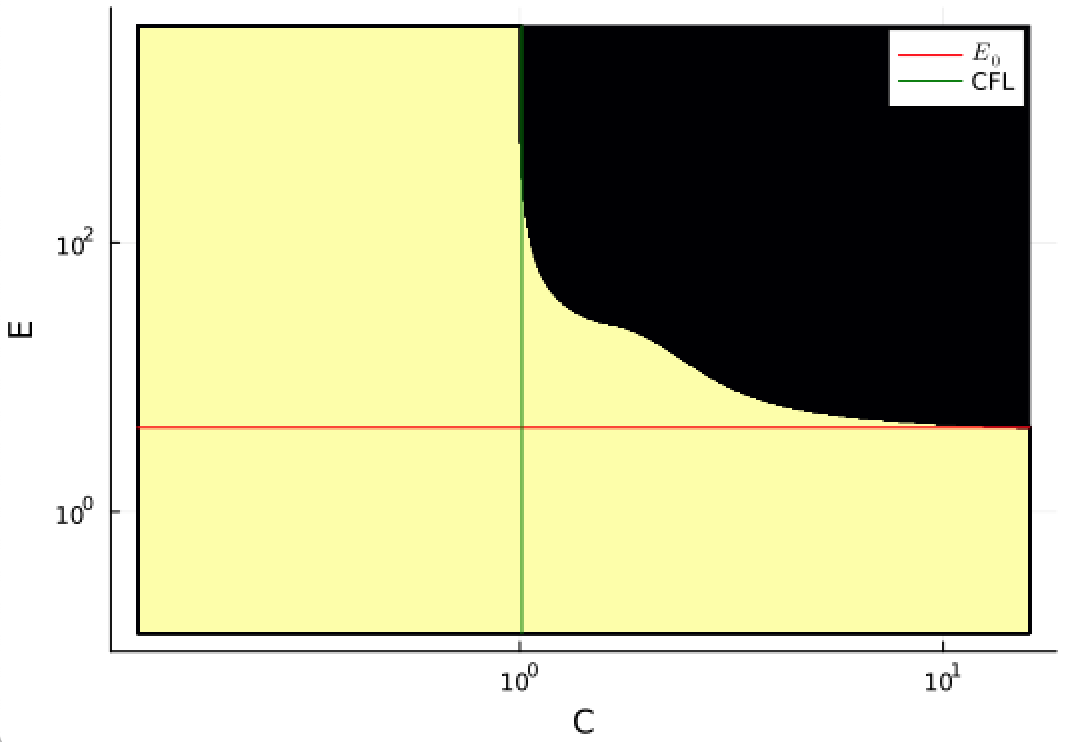
\includegraphics[width=\textwidth]{pdepics/IMEXsDeC2_GLB_diff2_adv1_C_log.png}
	\end{minipage} 
	\begin{minipage}[t]{0.45\textwidth}
		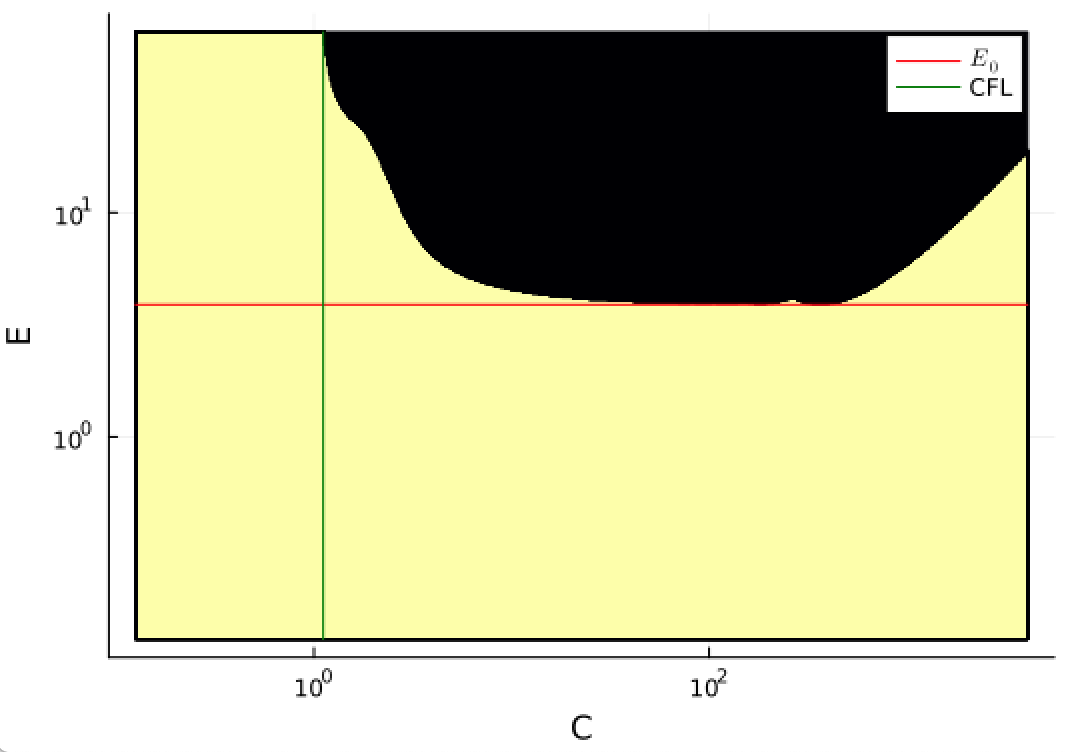
\includegraphics[width=\textwidth]{pdepics/IMEXsDeC2_GLB_diff2_adv1_E_log.png}
	\end{minipage}
	\caption{$[sDeC,GLB,2, A_1,D_2]$: Stability Behavior for large $C$ (left)and large $E$(right).}
	\label{fig: exa_limits}
\end{figure}

In figure \ref{fig: exa_advtermDeC} are the stability areas displayed for the $[DeC,eq,8, A_k,D_2]$ and $[DeC,eq,8, A_k,D_8]$ while increasing the order for the finite difference scheme for the advection part in different scenarios with $k$. Increasing the finite differences of the advection part does not result in higher values for $E_0$ and $C_0$, but seemingly decreases for odd orders and increases for even orders, while starting with relatively big values for order 1 and relatively small values for order 2. It seems that they all guide towards a specific border line. It is also outstanding that  we do not receive a border $E_0>0$ for order 6 in the advection term on the left, while we do on the right. These phenomena hold for all remaining combinations of time-marching methods, respective orders and nodes also, i.e. if we incease the order of the diffusion term, we can eliminate instabilities that occur due to the advection term, while the remaining variables just play a minor role. Exemplary, we display in figure \ref{fig: exa_advtermADER} on the left the $[ADER,GLB,8, A_k,D_2]$ and in the middle the $[ADER,eq,2, A_k,D_8]$ to underly this statement. The only exception we observed appears for the higher order ADER with equispaced nodes, as we already saw in figure \ref{fig: grp_adv1_diff2_eq} and is displayed for varying advection terms in figure \ref{fig: exa_advtermADER} on the right: Under these conditions, the instabilities remain.

\begin{figure}[!h]
	\centering
	\begin{minipage}[t]{0.33\textwidth}
		\includegraphics[width=\textwidth]{pdepics/IMEXDeC8_diff2_adv8_equispaced.png}
		\centering
		$[DeC,eq,8, A_k,D_2]$
	\end{minipage} 
	\begin{minipage}[t]{0.33\textwidth}
		\includegraphics[width=\textwidth]{pdepics/IMEXDeC8_diff8_adv8_equispaced.png}
		\centering
		$[DeC,eq,8, A_k,D_8]$
	\end{minipage}
	\caption{DeC Stability areas varying the order of the advection method.}
	\label{fig: exa_advtermDeC}
\end{figure}


\begin{figure}[!h]
	\centering
	\begin{minipage}[t]{0.32\textwidth}
		\includegraphics[width=\textwidth]{pdepics/IMEXADER8_diff2_adv8_gaussLobatto.png}
		\centering
		$[ADER,GLB,8, A_k,D_2]$
	\end{minipage} 
	\begin{minipage}[t]{0.32\textwidth}
		\includegraphics[width=\textwidth]{pdepics/IMEXADER2_diff8_adv8_equispaced.png}
		\centering
		$[ADER,eq,2, A_k,D_8]$
	\end{minipage}
	\begin{minipage}[t]{0.32\textwidth}
		\includegraphics[width=\textwidth]{pdepics/IMEXADER8_diff8_adv8_equispaced.png}
		\centering
		$[ADER,eq,8, A_k,D_8]$
	\end{minipage}
	\caption{ADER Stability areas varying the order of the advection method.}
	\label{fig: exa_advtermADER}
\end{figure}

In figure \ref{fig: exa_diffterm} is a rising of the finite differences order for the diffusion part shown for the $[j,eq, 8, A_1,D_k]$, where $j$ is every of the 3 considered methods and $k \in \{2,4,6,8\}$.  We observe that the stability areas of all methods vary slightly, but do not increase or decrease the stability region in a significant way. Just for the ADER with equispaced nodes, we observe the stability problems mentioned before. Note that they appear for every order, because we chose the time-marching order to 8. \\

\begin{figure}[!h]
	\centering
	\begin{minipage}[t]{0.32\textwidth}
		\includegraphics[width=\textwidth]{pdepics/IMEXDeC8_diff8_adv1_Iserles.png}
		\centering
		$[DeC,eq, 8, A_1,D_k]$
	\end{minipage} 
	\begin{minipage}[t]{0.32\textwidth}
		\includegraphics[width=\textwidth]{pdepics/IMEXDeC_subtimesteps8_diff8_adv1_Iserles.png}
		\centering
		$[sDeC,eq, 8, A_1,D_k]$
	\end{minipage}
	\begin{minipage}[t]{0.32\textwidth}
		\includegraphics[width=\textwidth]{pdepics/IMEXADER8_diff8_adv1_Iserles.png}
		\centering
		$[ADER,eq, 8, A_1,D_k]$
	\end{minipage}
	\caption{Stability areas varying the order of the diffusion method.}
	\label{fig: exa_diffterm}
\end{figure}

In figure \ref{fig: exa_difftermsim}, we present a variation to figure \ref{fig: exa_diffterm} by matching the orders of the time-marching method with the order of the central difference for the diffusion term, i.e.  $[j,eq, k, A_1,D_k]$, where $j$ is every of the 3 considered methods and $k \in \{2,4,6,8\}$.
Here, we can observe for all cases that the higher order terms results in slightly larger stability areas and also in bigger $C_0$ and $E_0$, which leads back to the effects we have already seen for the time-marching method. Further, we observe that the ADER method  of order 8 with Gauss-Lobatto nodes does not produce instabilities here, as expected.\\

\begin{figure}[!h]
	\centering
	\begin{minipage}[t]{0.32\textwidth}
		\includegraphics[width=\textwidth]{pdepics/IMEXDeC8_diff8_adv1_gaussLobatto.png}
		\centering
		$[DeC,eq, k, A_1,D_k]$
	\end{minipage} 
	\begin{minipage}[t]{0.32\textwidth}
		\includegraphics[width=\textwidth]{pdepics/IMEXDeC_subtimesteps8_diff8_adv1_gaussLobatto.png}
		\centering
		$[sDeC,eq, k, A_1,D_k]$
	\end{minipage}
	\begin{minipage}[t]{0.32\textwidth}
		\includegraphics[width=\textwidth]{pdepics/IMEXADER8_diff8_adv1_gaussLobatto.png}
		\centering
		$[ADER,eq, k, A_1,D_k]$
	\end{minipage}
	\caption{Stability areas varying the order of the diffusion method.}
	\label{fig: exa_difftermsim}
\end{figure}

We can conclude that increasing the order of the time-marching method results in higher values for both $C_0$ and $E_0$. However, the here considered higher order finite differences for the spatial discretizations do not grant significant improvements. In the recent analysis, the border $E_0$ vanishes for the special setting IMEX ADER of order $>7$  with equispaced nodes, independent of the spatial discretization we used. We also receive this phenomenon by setting the advection method to order 6, but this problem can be overcome by the usage of high order diffusion methods.\\
Remark also, that there are plenty more options to test, which we leave out because of space. Nevertheless, we presented all remarkable cases and other combinations of methods were tested and lead to similar results.

\subsection{Advection--dispersion equations}
In this section, we want to extend the used analysis and results to observe the behavior of IMEX ADER and DeC methods onto the advection-dispersion equation
\begin{equation}
\label{eq: A-Disp_equation}
u_t(x,t) + au_x(x,t) + d_pu_{xxx}(x,t) = 0, \quad a\ge0, \ d_p \ge 0.
\end{equation}
\subsubsection{FD discretization}
\label{sec: disp_spatial_discretization}
Similar to the advection-diffusion equation, we want to introduce at this point the considered spatial discretizations for the advection-dispersion equation. Thereby, we will consider the same schemes for the advection term, as introduced in section \ref{sec: spatial_discretization}.\\
For the dispersion term, we will take two different types of methods into account: Central finite difference schemes and upwind schemes. The underlying theory and assumptions are the same as we saw previously and their orders can be proven analogue. The central finite difference schemes can be found in figure \ref{fig: CFD-schemes_third_deriv}.
\begin{figure}
	\centering
	\small
	\begin{tabular}[h]{|c|c|}
		\hline
		order & finite difference for $\partial_h^3(u(x_j))$\\
		\hline
		2&$ \frac{1}{h^3}\left(-\frac{1}{2}w_{j-2} + w_{j-1} - w_{j+1} + \frac{1}{2}w_{j+2}\right)$ \\
		\hline
		4 & $\frac{1}{h^3}\left(\frac{1}{8} w_{j-3} - w_{j-2} + \frac{13}{8}w_{j-1} - \frac{13}{8}w_{j+1} + w_{j+2} - \frac{1}{8}w_{j+3}\right)$\\
		\hline
		6 & $\frac{1}{h^3}\left(-\frac{7}{240}w_{j-4} + \frac{3}{10}w_{j-3} - \frac{169}{120}w_{j-2} + \frac{61}{30}w_{j-1} - \frac{61}{30}w_{j+1} + \frac{169}{120}w_{j+2} - \frac{3}{10}w_{j+3} + \frac{7}{240}w_{j+4}\right)$\\
		\hline
	\end{tabular}
	\caption{Central finite difference discretizations $w_j$ approximating $u(x_j)$, \cite{fornberg_finite_difference}.}
	\label{fig: CFD-schemes_third_deriv}
\end{figure}
We will consider the upwind scheme, taken out of \cite{TanChenShu_ImEx_Stability}, where they also use it to test stability for the advection-dispersion equation. It is of order 3 and given by
\begin{equation}
\label{eq: shu_upwind_dispersion}
\partial_h^3(u(x_j)) =\frac{1}{4h^3}\left( -w_{j-2} - w_{j-1}  + 10w_{j} - 14w_{j+1} + 7w_{j+2} - w_{j+3}\right).
\end{equation}

\subsubsection{von Neumann Stability}
As done previously, we will perform von Neumann analysis by looking at the coefficients of the finite difference schemes, i.e. $C=a\frac{\Delta t}{\Delta x}$ and $D_p= d_p\frac{\Delta t}{{\Delta x}^3}$. So technically, we compute the methods in the same way and just adapt the spatial schemes from the diffusion term to the dispersion term. Remark that also the sign of this term gets changed. 
\subsubsection{Displaying stability}
We introduce a similar notation:
\LP{As before determined, write down here the notation}
\begin{definition}\mbox{}\\
	The considered method for the advection-dispersion equation will be denoted by
	\begin{equation*}
	[TMM,NODES,N, A_n,D_n],
	\end{equation*}
	where
	\begin{itemize}
		\item $TMM$stands for the respective IMEX time-marching method, i.e. $DeC$, $ADER$, $DeC$,
		\item $NODES$ stands for the used quadrature nodes for the TMM, i.e. $eq$ for equispaced or $GLB$ for Gauss-Lobatto,
		\item $N$ stands for the order of the considered time-marching method $TMM$,
		\item $A_n$ denotes order $n$ for the optimal-order stable stencils of proposition \ref{prop: optimal_order_stable} used for the advection part and
		\item $D_m$ denotes order $m$ for the central finite differences \ref{fig: CFD-schemes_third_deriv}, with the speacial case $m==u$, if we use the upwind method \ref{eq: shu_upwind_dispersion} used for the dispersion part.
	\end{itemize}
\end{definition}
We proceed by utilizing the experience of chapter \ref{sec: advection_diffusion}, and evaluate the amplification factor 
\begin{equation*}
g=g(k,\Delta x, \Delta t, a, d_p)=g(k,C,D_p)
\end{equation*}
to observe where we are stable in dependence of $C$ and $D_p$. Note that we do not have any outlines or further goals considering a spatial-independent condition, as we had for the advection-dispersion with \cite{TanChenShu_ImEx_Stability}. Instead, we will just observe and hope for some similar results.\\
For that matter we define the coefficients:
\begin{equation*}
C:= \frac{a\Delta t}{\Delta x}, \quad D_p := \frac{d_p \Delta t}{(\Delta x)^3}
\end{equation*}
and also take the analouge appraoch into consideration, by defining
\begin{equation*}
E_p:=\frac{C^3}{D_p}=\frac{\Delta t^3a^3}{\Delta x^3}\frac{\Delta x^3}{d_p\Delta t}=\frac{a^3}{d_p}\Delta t
\end{equation*}
with the similar hope, to find some $c$ for each method, such that $E_p\le c$. Then, we have a spatial-independent time-step restriction.\\
\begin{example}\label{exa: disp_displaying_stability}\mbox{}\\
	In figure \ref{fig: disp_IIMEXDeC2/3_GLB_CvsD} are the stability areas displayed for the $[DeC, EQ,2,A_1, D_2]$ and \\$[DeC, EQ,3,A_1, D_2]$ in dependence of $C$ and $D_p$.
	\begin{figure}[!h]
		\centering
		\begin{minipage}[t]{0.24\textwidth}
			\centering
			\includegraphics[width=\textwidth]{pdepics/disp/disp_IMEXDeC2_gaussLobatto_adv1_disp2.png}
			IMEX DeC2
		\end{minipage} 
		\begin{minipage}[t]{0.24\textwidth}
			\centering
			\includegraphics[width=\textwidth]{pdepics/disp/disp_IMEXDeC2_gaussLobatto_adv1_disp2_far.png}
			IMEX DeC2 (zoomed)
		\end{minipage}
		\begin{minipage}[t]{0.24\textwidth}
			\centering
			\includegraphics[width=\textwidth]{pdepics/disp/disp_IMEXDeC3_gaussLobatto_adv1_disp2.png}
			IMEX DeC3
		\end{minipage}
		\begin{minipage}[t]{0.24\textwidth}
			\centering
			\includegraphics[width=\textwidth]{pdepics/disp/disp_IMEXDeC3_gaussLobatto_adv1_disp2_far.png}
			IMEX DeC3 (zoomed)
		\end{minipage}
		\caption{Stability areas for example \ref{exa: disp_displaying_stability}: $C$ against $D_p$.}
		\label{fig: disp_IIMEXDeC2/3_GLB_CvsD}
	\end{figure}
	In all cases, we do not observe a presumable quadratic behavior between the stable and unstable region, but instead an CFL-like behavior which passes over into larger possible values for $C$, if $D_p$ is $"$large$"$. Note that $D_p$ still depends on $\Delta x$. For order 3, we detect in addition an unstable region, evolving for lager $D_p$ and low $C$ together.\\
	Shifting onto an evaluation of $C$ against $E_p$, as displayed in figure \ref{fig: disp_IIMEXDeC2/3_GLB_CvsE}, we can also observe worse results than for the advection-diffusion equation: Besides of the similar behavior to the advection-diffusion stability areas, we can firstly remark that especially the $E_0$-border is much smaller and that we receive instability again for very small $E_0$.\\
	\begin{figure}[!h]
		\centering
		\begin{minipage}[t]{0.24\textwidth}
			\centering
			\includegraphics[width=\textwidth]{pdepics/disp/disp_IMEXDeC2_gaussLobatto_adv1_disp2_EDP.png}
			IMEX DeC2
		\end{minipage} 
		\begin{minipage}[t]{0.24\textwidth}
			\centering
			\includegraphics[width=\textwidth]{pdepics/disp/disp_IMEXDeC2_gaussLobatto_adv1_disp2_EDP2.png}
			IMEX DeC2 (zoomed)
		\end{minipage}
		\begin{minipage}[t]{0.24\textwidth}
			\centering
			\includegraphics[width=\textwidth]{pdepics/disp/disp_IMEXDeC3_gaussLobatto_adv1_disp2_EDP.png}
			IMEX DeC3
		\end{minipage}
		\begin{minipage}[t]{0.24\textwidth}
			\centering
			\includegraphics[width=\textwidth]{pdepics/disp/disp_IMEXDeC3_gaussLobatto_adv1_disp2_EDP2.png}
			IMEX DeC3 (zoomed)
		\end{minipage}
		\caption{Stability areas for example \ref{exa: disp_displaying_stability}: $C$ against $E_p$.}
		\label{fig: disp_IIMEXDeC2/3_GLB_CvsE}
	\end{figure}
	
	These exemplary stability regions hold for most of the considered cases, i.e. all methods of order 2 do not have the instability areas for small $C$ and large $D_p$, as well as the IMEX ADER methods with equispaced nodes until order 4 and all IMEX ADER methods with Gauss-Lobatto nodes. Remark that these are exactly the methods which seem to be A-stable in their implicit ODE application as discussed in chapter \ref{sec: stability_analysis_ODE}. The remaining methods all possess this unfavorable stability region. Further, it can be observed that the instability areas for very small $E_0$ appear for much smaller $E_0$ if the belonging implicit ODE method is A-stable. This can be seen in the previous example and extends to all remaining considered methods. \\
\end{example}
Note also that we tested other coefficients, for example $C$ vs $\frac{C^2}{D_p}$ and did not recognize any favorable restrictions in terms of regularity or borders, as for the advection-diffusion equation. Higher order central differences for the dispersion term also do not result in stability improvements.\\
\subsubsection{Results for Implicit-Explicit DeC, sDeC and ADER}
In this section, we want to present most of the results we made for the analysis as displayed in example \ref{exa: disp_displaying_stability}. Based on this, we make the effort to increase stability by using various upwind biased methods for the dispersion term. The results were all similar, for which reason we will just proceed with the upwind method introduced in \eqref{eq: shu_upwind_dispersion}.
\begin{example}\label{exa: disp_displaying_stability_upwind}\mbox{}\\
	In figure \ref{fig: disp_IIMEXDeC2/3_GLB_CvsE_upwind} are the stability areas displayed for the $[DeC, eq,2,A_1,D_u]$ and \\$[DeC, eq,3, A_1,D_u]$ to compare the results to example \ref{exa: disp_displaying_stability}.
	As we can observe in a qualitative manner, we increase the stability mostly. The $C_0$ borders seem to increase, while we receive a completely different curve shape (again some quadratic-like) for the border of the stable and unstable region in the $C$ vs $D_p$ view. Also, the unstable regions on the top-left are shrinking even though they do not vanish at all. Nevertheless, we can not observe some improvements considering the unstable area for small $E_p$.
	\begin{figure}[!h]
		\centering
		\begin{minipage}[t]{0.45\textwidth}
			\centering
			\includegraphics[width=\textwidth]{pdepics/disp/disp_IMEXDeC2_gaussLobatto_adv1_upwind_EDP.png}
			IMEX DeC2
		\end{minipage} 
		\begin{minipage}[t]{0.45\textwidth}
			\centering
			\includegraphics[width=\textwidth]{pdepics/disp/disp_IMEXDeC2_gaussLobatto_adv1_upwind_EDP_small.png}
			IMEX DeC2 (zoomed)
		\end{minipage}
		\begin{minipage}[t]{0.45\textwidth}
			\centering
			\includegraphics[width=\textwidth]{pdepics/disp/disp_IMEXDeC3_gaussLobatto_adv1_upwind_EDP.png}
			IMEX DeC3
		\end{minipage}
		\begin{minipage}[t]{0.45\textwidth}
			\centering
			\includegraphics[width=\textwidth]{pdepics/disp/disp_IMEXDeC3_gaussLobatto_adv1_upwind_EDP_small.png}
			IMEX DeC3 (zoomed)
		\end{minipage}
		\begin{minipage}[t]{0.45\textwidth}
			\centering
			\includegraphics[width=\textwidth]{pdepics/disp/disp_IMEXDeC2_gaussLobatto_adv1_upwind.png}
			IMEX DeC2 ($C$ and $D_p$)
		\end{minipage}
		\begin{minipage}[t]{0.45\textwidth}
			\centering
			\includegraphics[width=\textwidth]{pdepics/disp/disp_IMEXDeC3_gaussLobatto_adv1_upwind.png}
			IMEX DeC3 ($C$ and $D_p$)
		\end{minipage}
		\caption{Stability areas for $[DeC, eq,2,A_1, D_u]$ and $[DeC, eq,2,A_1, D_u]$.}
		\label{fig: disp_IIMEXDeC2/3_GLB_CvsE_upwind}
	\end{figure}
\end{example}
In the following, we will present the stability results for remaining, mentionable cases by looking at the coefficients $C$ vs $E_p$ while using the before considered upwind method for the dispersion term. To distinguish the different orders, we apply different colors to the outer and inner bounds according to the legend \ref{fig: legend_disp}. Remark that the colors are assigned to different types of orders, i.e. in one figure to the order of the time-marching method, in the other one to the order of the advection method.
\begin{figure}[!h]
	\centering
	\includegraphics[width=0.18\textwidth]{pdepics/disp/colors_disp.png}
	\caption{Legend for the different orders.}
	\label{fig: legend_disp}
\end{figure}\\

In figure \ref{fig: disp_allRK_GLB}, we can observe the behavior for increasing the order of the respective ODE method from 2 to 6. 
We see again that all the DeC methods do not provide an $E_{p_0}$ border due to the before mentioned effects, but some border $C_0\approx 2$ for every method. The same holds for the ADER methods, while we can observe some more unstable behavior for small $E_p$. Additionally, we observe an unusual loss of stability for the $[ADER, GLB, 2 A_1, D_u]$. We can also observe smaller borders $C_0$ than for the DeC methods. For the sDeC, we have similar values for $C_0$, while for orders over 2 the border curve seems to be located over some much larger border line $E_{p_0}$ than for the other methods: While DeC and ADER seem to have $E_{p_0}$ border values around $E_p=0.1$, the sDeC has values over 5 for orders over 2, increasing with order. We also note that the anticipated $E_{p_0}$ borders change for different orders and may take similar values as for $E_0$ in the advection-diffusion case. Nevertheless, the minor instability regions below exist as it can be seen in figure \ref{fig: sDeC4_adv1_upwind_large} for the IMsDeC order 4. For this reason, we can not assign them spatial-independent stability conditions $E_{p_0}$. 
\begin{figure}[!h]
	\centering
	\begin{minipage}[t]{0.32\textwidth}
		\centering
		\includegraphics[width=\textwidth]{pdepics/disp/IMEXDeC6_gaussLobatto_adv1_upwind.png}
		\small$[DeC, GLB,k, A_1,D_u]$\par
	\end{minipage}
	\begin{minipage}[t]{0.32\textwidth}
		\centering
		\includegraphics[width=\textwidth]{pdepics/disp/IMEXADER6_gaussLobatto_adv1_upwind.png}
		\small$[ADER, GLB,k, A_1,D_u]$\par
	\end{minipage}
	\begin{minipage}[t]{0.32\textwidth}
		\centering
		\includegraphics[width=\textwidth]{pdepics/disp/IMEXDeC_subtimesteps6_gaussLobatto_adv1_upwind.png}
		\small$[sDeC, GLB,k, A_1,D_u]$\par
	\end{minipage}
	\caption{Stability areas for orders 2 to 6 with GaussLobatto nodes, the upwind scheme of \eqref{eq: shu_upwind_dispersion} for the dispersion and an first order backward scheme for the advection term.}
	\label{fig: disp_allRK_GLB}
\end{figure}

\begin{figure}[!h]
	\centering
	\includegraphics[width=0.48\textwidth]{pdepics/disp/disp_sDeC4_adv1_upwind_EDP_large.png}
	\caption{The sDeC4 method with GaussLobatto nodes displayed on an larger scale.}
	\label{fig: sDeC4_adv1_upwind_large}
\end{figure}

In figure \ref{fig: disp_allRK_EQ}, we showcase the same methods as before, but using equispaced nodes. We observe no mentionable differences except for the ADER method, where we receive different shapes of instabilities for small $E_p$, resulting in $C_0=0$ for order 6. This reminds of the ADER method for the advection-diffusion equation, where we also observed iinstabilities for higher orders.  Further, we could observe that the instabilities we receive for both small $E_p$ and small $C$ are not only small for order 2, but also for higher orders in the ADER case with Gauss-Lobatto nodes and also with equispaced nodes until order 4.  As already mentioned before, this could also be a result of the loss of A-stability for the certain order of the IMADER with equispaced nodes. 
\begin{figure}
	\begin{minipage}[t]{0.32\textwidth}
		\centering
		\includegraphics[width=\textwidth]{pdepics/disp/IMEXDeC6_equispaced_adv1_upwind.png}
		\small$[DeC, eq,k,A_1,D_u]$\par
	\end{minipage}
	\begin{minipage}[t]{0.32\textwidth}
		\centering
		\includegraphics[width=\textwidth]{pdepics/disp/IMEXADER6_equispaced_adv1_upwind.png}
		\small$[ADER, eq,k, A_1,D_u]$\par
	\end{minipage}
	\begin{minipage}[t]{0.32\textwidth}
		\centering
		\includegraphics[width=\textwidth]{pdepics/disp/IMEXDeC_subtimesteps6_equispaced_adv1_upwind.png}
		\small$[sDeC, eq,k, A_1,D_u]$\par
	\end{minipage}
	\caption{Stability areas for orders 2 to 6 with equispaced nodes, the upwind scheme of \eqref{eq: shu_upwind_dispersion} for the dispersion and an first order scheme for the advection term.}
	\label{fig: disp_allRK_EQ}
\end{figure}


In figure \ref{fig: disp_alladv_GLB}, we can observe the behavior by increasing the order of the stable advection stencils exemplary for the DeC and ADER methods with Gauss-Lobatto nodes. We find a loss of stability by increasing the order. We already see a slight reduction of our border $C_0$ for order 2 and 3. Going onto orders 4, 5 and 6, the anticipated border $C_0$ gets reduced by a factor in the range of $10^3$. Remark that we get instabilities in the region around $C=0, E_p=0$ for the ADER case, which we do not have for the DeC case. We also tried out to match the orders of the advection scheme and the time-marching method. This lead to some minor improvements, but did not remove the issues of higher order advection methods as we can observe here.
\\
We spare out the remaining cases again to not exaggerate the number of plots. Further, we also checked the result for other nodes and the sDeC and they were similar in their stability behavior (sDeC similar to DeC). 
\begin{figure}
	\begin{minipage}[t]{0.45\textwidth}
		\centering
		\includegraphics[width=\textwidth]{pdepics/disp/IMEXDeC2_gaussLobatto_adv6_upwind.png}
		\small$[DeC, GLB,2,A_k,D_u]$\par
	\end{minipage}
	\begin{minipage}[t]{0.45\textwidth}
		\centering
		\includegraphics[width=\textwidth]{pdepics/disp/IMEXADER2_gaussLobatto_adv6_upwind.png}
		\small$[ADER, GLB,2,A_k,D_u]$\par
	\end{minipage}
	\\
	\begin{minipage}[t]{0.45\textwidth}
		\centering
		\includegraphics[width=\textwidth]{pdepics/disp/IMEXDeC2_gaussLobatto_adv6_upwind_zoom.png}
		\small$[DeC, GLB,2,A_k,D_u]$(zoomed)\par
	\end{minipage}
	\begin{minipage}[t]{0.45\textwidth}
		\centering
		\includegraphics[width=\textwidth]{pdepics/disp/IMEXADER2_gaussLobatto_adv6_upwind_zoom.png}
		\small$[ADER, GLB,2,A_k,D_u]$(zoomed)\par
	\end{minipage}
	\caption{Stability areas varying orders 2 to 6 of the advection scheme.}
	\label{fig: disp_alladv_GLB}
\end{figure}


We conclude that the here observed IMEX methods combined with the finite difference stencils for the spatial discretization do not possess fully a spatial-independent condition on the time step. For many of the methods with an A-stable implicit ODE part, these lower time step restrictions are so weak that it may not have an effect in many applications, especially because the dispersion coefficient $d_p$ uses to be small, which makes the time step controllable. Nevertheless, we can not rely on this further. The border $C_0$ is also affected by that matter. But because of the really small effects of the before mentioned methods with the A-stable implicit ODE part, we assume that it does not affect the stability significantly. In further terms of stability, upwind schemes for the dispersion term perform better than central schemes, while increasing the order of the advection stencils also goes with a loss. Especially for the ADER methods with order $\le 3$, these stencils go with problematic instabilities.